\citer{
\textbf{Architecture} : 1. Art, science et technique de la construction, de la
restauration, de l'am\'enagement des \'edifices. \emph{P. anal.} 
1. Principe d'organisation d'un ensemble, agencement, structure :
2. Ensemble structur\'e, organis\'e, construction \emph{Rem.} 1. Le
terme est employ\'e, tant sur le plan concr. que sur le plan abstr.,
dans des cas tr\`es divers o\`u il y a agencement, combinaison de
diff\'erentes parties pour former un tout, un ensemble homog\`ene,
organis\'e (ou paraissant l'\^etre) selon une certaine structure, un
certain plan. \'ETYMOL. ET HIST. Empr. au lat. architectura \og art
de construire \fg}{Tr\'esor de la Langue Fran\c{c}aise}


Nous avons dans le chapitre \ref{cha:proc-de-devol} insist\'e sur le
besoin d'une conception formalis\'ee de l'architecture des
logiciels. Nous avons aussi conclu que la notion d'architecture
\'etait li\'ee \`a la notion de composants. Ce chapitre sera donc
consacr\'e \`a ce qu'il est convenu d'appeler
l'\'etat de l'art dans le domaine de la mod\'elisation, de la
sp\'ecification et de la r\'ealisation d'architecture de syst\`emes
\`a base de composants.

Nous partirons des outils et plateformes orient\'ees-composant
concr\`etes, dans lesquelles un composant est une entit\'e
logicielle bien d\'efinie, s'ins\'erant dans un mod\`ele
d'ex\'ecution et de communication lui aussi pr\'ecis. Le
d\'eveloppement sur ces plateformes --- \textsf{J2EE},
\textsf{Corba}, \textsf{.Net} ---  constituent aujourd'hui l'essentiel
des d\'eveloppements dans les soci\'et\'es de services. Et nous
essayerons de comprendre pourquoi ces plateformes sont un \'echec
relatif en termes d'am\'elioration de la qualit\'e des logiciels. 

Ceci nous am\'enera naturellement \`a \'etudier un certain nombre
de propositions pour la conception d'architectures. \`A partir des
outils de mod\'elisation propos\'es autour du langage \textsf{UML},
nous nous int\'eresserons plus particuli\`erement aux nombreux travaux autour des \emph{Langages de
  Description d'Architecture} --- \textsf{ADL} en anglais. Sachant
qu'il existe d\'ej\`a des excellentes synth\`eses sur les ADL les
plus anciens, nous nous concentrerons sur quelques propositions plus 
r\'ecentes du domaine.

Enfin, nous aborderons certains mod\`eles plus th\'eoriques qui
s'int\'eressent \`a la composition de composants poss\'edant une
description comportementale formalis\'ee. 

\section{Plateformes de composants}

Une d\'efinition tr\`es fr\'equemment reprise du terme de composant
est celle propos\'ee  dans \cite{szyperski} (p.36, traduction par nos
soins) : 
\begin{quote}
    \og Un composant logiciel est une unit\'e de composition avec des
    interfaces contractuellement sp\'ecifi\'ees et des
    d\'ependances uniquement contextuelles. Un composant logiciel
    peut \^etre d\'eploy\'e de mani\`ere ind\'ependante et
    compos\'e par des \'el\'ements tiers. \fg
\end{quote}
Cette d\'efinition est
ax\'ee comme l'ensemble de l'ouvrage cit\'e sur une vision
essentiellement \emph{technologique} et \'economique de la notion de
composants :  le 
probl\`eme consid\'er\'e est celui de la construction de logiciels \`a partir de
composants r\'eutilisables et du d\'eveloppement subs\'equent d'un
\emph{march\'e} de composants. 

Cette premi\`ere partie pr\'esente les outils r\'epondant \`a cette d\'efinition : les
\emph{plateformes \`a composants} ou \emph{intergiciels \`a
  composants}. Trois acteurs de taille in\'egale se partagent
aujourd'hui ce march\'e : \textsf{Java} et \textsf{J2EE} qui en
poss\`ede la plus grand part,  \textsf{.Net} qui est la r\'eponse de
\textsc{Microsoft} et qui prend de l'ampleur, et \textsf{Corba} et le
\emph{Corba Component Model} --- ou \textsf{CCM} --- qui est
conceptuellement la meilleure proposition des trois mais qui reste
marginale. Nous incluerons dans cette cat\'egorie \textsf{Fractal}
qui se pr\'esente comme une plateforme de composants, bien qu'elle ne
soit pas encore pr\'esente dans le domaine des services logiciels. 

La seconde partie de cette section s'int\'eressera \`a des
technologies plus r\'ecentes et moins ambitieuses qui visent \`a
pallier \`a la grande complexit\'e de mise en \oe uvre des
intergiciels. Ces technologies sont g\'en\'eralement inspir\'ees
des \emph{langages de configuration} et offrent essentiellement un \emph{cadre
m\'ethodologique} bas\'e sur la notion de composants.

\subsection{Intergiciels \`a composants}

Les intergiciels sont n\'es de  la volont\'e
de r\'esoudre le probl\'eme de la \emph{distribution} des applications sur
un ensemble de syst\`emes interconnect\'es par un
r\'eseau. L'objectif initial et \`a ce jour non atteint \'etait de
rendre \emph{transparente} pour le d\'eveloppeur et l'utilisateur la
structure r\'epartie des applications. Pour le d\'eveloppeur, il
s'agissait par ailleurs de faciliter le d\'eveloppement, le
d\'eploiement et la maintenance de telles applications. Les intergiciels
que nous \'etudions ici ne constituent qu'une r\'eponse parmi
d'autres possibles \`a ce probl\`eme et l'on trouvera dans
\cite{tannenbaum-dist-syst} une introduction compl\`ete et accessible
sur les autres solutions techniques \`a ce probl\`eme. 

\subsubsection{J2EE}
\label{sec:j2ee}

\textsf{J2EE}, pour \emph{Java 2 Enterprise Edition}  est une
extension de l'\textsf{API Java}
sp\'ecifiquement destin\'ee \`a la r\'ealisation de \emph{syst\`emes
d'informations d'entreprises}. Les d\'eveloppements vis\'es sont
des syst\`emes autonomes ou plus souvent des sous-syst\`emes collaborant avec d'autres
sous-syst\`emes tels que des base de donn\'ees, des applications
patrimoniales client-serveur ou en sites centraux, des
\textsf{ERP}. \textsf{J2EE}, actuellement dans sa version 1.4, est \`a la fois une norme pour les concepteurs de
plateformes et d'outils et en ensemble d'API pour les
d\'eveloppeurs d'application.  Le site \emph{Web} de \textsc{Sun} est
bien entendu la r\'ef\'erence sur cette plateforme\cite{ejbspec,j2eespec}. 

\paragraph{Caract\'eristiques}

Nous ne rentrerons pas dans le d\'etail de l'architecture de la
plateforme \textsf{J2EE} et nous contenterons d'en souligner les
principales caract\'eristiques.

Le support d'ex\'ecution d'une application \textsf{J2EE} est le \emph{serveur
d'application}
destin\'e \`a lier les diff\'erents composants de l'application
entre eux. Le conteneur offre aussi des interfaces sp\'ecifiques vers
les services techniques de la plateforme. Diff\'erents types de
composants sont support\'es par \textsf{J2EE} :  les composants
\emph{Web} tels que  \emph{servlets} et \emph{Java Server Pages} ; les composants \textsf{EJB} --- \emph{Enterprise JavaBeans} --- ou
  composants m\'etiers ; les \emph{connecteurs} vers des syst\`emes
  externes ; les applications autonomes.

L'unit\'e de d\'eploiement du composant est l'\emph{archive}
accompagn\'ee de son \emph{descripteur de d\'eploiement}. Elle peut
en th\'eorie \^etre d\'eploy\'ee sur n'importe quel serveur 
d'application  conforme \`a la sp\'ecification \textsf{J2EE}. Une application constitu\'ee d'un ensemble
de composants peut \^etre empaquet\'ee et d\'eploy\'ee globalement.  

Le concept de \emph{conteneur} permet aux composants de s'abstraire
des d\'etails techniques de la gestion du contexte d'ex\'ecution et
offre un point d'acc\`es \`a divers services normalis\'es :
l'invocation de m\'ethodes distantes ou \textsf{RPC} ; le
\emph{service de nommage} ; le \emph{service de gestion des
  transactions}  ; la \emph{gestion de la persistence} ; la
\emph{messagerie asynchrone} ; la gestion du \emph{cycle de vie} des composants en fonction de leur
  nature. L'acc\`es \`a ces service se fait soit au travers d'une
  \textsf{API} offerte par le conteneur, soit par d\'eclaration dans
  un descripteur ad-hoc.

Les \textsf{EJB} constituent les composants m\'etiers d'une
application \textsf{J2EE} : ce sont eux qui contiennent les
traitements \`a r\'ealiser et qui r\'ealisent l'interface entre les
donn\'ees persistantes et la logique de pr\'esentation de
l'application (voir chapitre \ref{cha:proc-de-devol}, section
\ref{sec:arch-logic}). 
Les composants \textsf{EJB} sont r\'epartis en trois cat\'egories : 
\begin{itemize}
  \item les \emph{EJB Session} n'ont pas d'identit\'e propre au
    del\`a d'une invocation ou d'une s\'equence d'invocations de
    m\'ethodes ; 
  \item les \emph{EJB Entit\'e} ont une identit\'e persistante : ils
  repr\'esentent des informations m\'etiers stock\'ees dans une
  base le plus souvent relationnelle ;
  \item les \emph{EJB Message} r\'ealisent des traitements
  asynchrones d\'eclench\'es \`a partir de files de messages. 
\end{itemize}

\paragraph{Critiques}

Les critiques de la section \ref{sec:analyse-critique} ne sont pas
toutes dues au processus de d\'eveloppement. Une partie non
n\'egligeable du probl\`eme a sa source dans la complexit\'e de la
plateforme utilis\'ee, en l'occurence \textsf{J2EE}. Cette plateforme
n'est pas en effet r\'eellement une plateforme \`a base de
composants mais plut\^ot une solution technique orient\'ee-objet
pour les syst\`emes r\'epartis. Cette solution n'est pas
n\'ecessairement mauvaise, mais appuyer une conception sur une telle
structure ne peut que noyer le mod\`ele architecturale dans trop de
d\'etails. Et les outils existant ne parviennent pas \`a masquer
suffisamment cette complexit\'e pour permettre de s'en abstraire.

\subsubsection{\textsf{.Net}}
\label{sec:.net}
La plateforme \textsf{.Net} est la r\'eponse de \textsc{Microsoft} au
d\'eveloppement des applications Java dans les syst\`emes
d'information d'entreprise. Elle constitue une refonte compl\`ete de
l'architecture \textsf{COM/DCOM/ActiveX}  existant depuis de nombreuses
ann\'ees sur le syst\`eme Windows et qui avait d\'ej\`a pour
objectif de faciliter la communication entre applications, locales
puis distantes, et le d\'eveloppement d'un march\'e de composants
r\'eutilisables essentiellement dans le domaine des interfaces
graphiques.

Nous nous basons pour cette \'etude sur \cite{szyperski}, chapitre
15, consacr\'e \`a la vision de \textsc{Microsoft} de la notion de
composants et sur \cite{lantin-dotnet} qui est une synth\`ese des
techniques de programmation sur plateforme  \textsf{.Net}. Rappelons
par ailleurs que les travaux sur
\textsf{AsmL}\cite{gurevich-asml-semantic,barnett-asm-components}  ont
pour cible la formalisation de composants et d'architectures \textsf{.Net}.

Les caract\'eristiques principales de \textsf{.Net} sont les suivantes :
\begin{itemize}
  \item une infrastructure de langage commune --- \emph{Common Language
  Infrastructure}, \textsf{CLI} --- dont la sp\'ecification est
  publique et qui comprend :
  \begin{itemize}
    \item la d\'efinition d'un language interm\'ediaire
      ind\'ependant des langages de programmation de haut-niveau,
    \item un syst\`eme de types suffisamment riche pour supporter la
      plupart des concepts objets, 
    \item une sp\'ecification des
      assemblages, c'est \`a dire des applications ou composants de
      services 
    \item et un ensemble de m\'eta-informations accessibles \`a
      l'ex\'ecution et qui permet en particulier de r\'esoudre le
      probl\`eme des \emph{versions} d'interfaces, probl\`eme
      r\'ecurrent sous Windows plus connu sous le nom d'\og enfer des
      DLL\fg.
\end{itemize}
Cette infrastructure est similaire au JDK dans le monde
  Java et cette similarit\'e va jusqu'\`a l'implantation dans le
  \emph{Common Language Runtime}, c'est \`a dire la plateforme
  concr\`ete de Microsoft implantant le \textsf{CLI}, d'un compilateur
  \emph{Just-In-Time} afin que les applications puissent s'ex\'ecuter
  \`a la vitesse du code natif ;
\item les \emph{assemblages} qui sont l'unit\'e de base de
  d\'eploiement et qui poss\`edent la propri\'et\'e de disposer
  d'un nom symbolique qui est globalement unique. Les assemblages peuvent d\'efinir des
  d\'ependances explicites et des interfaces offertes, autrement dit
  ce sont d'authentiques composants. Le \textsf{CLR} et le syst\`eme d'exploitation
  sont responsables de la r\'ealisation effective des assemblages et
  donc de l'instantiation des composants et de la r\'esolution de
  leurs d\'ependances ;
\item l'int\'egration dans un framework de composants de services
  standards permettant d'acc\'eder \`a l'ensemble de l'\textsf{API} Windows ;
\item l'invocation distante de m\'ethodes soit au travers des
  m\'ecanismes \textsf{COM/DCOM/COM}+, soit bas\'ee sur les \emph{Web
  Services}. Dans le premier cas, les applications b\'en\'eficient
  de l'ensemble de l'infrastructure d\'evelopp\'ee au fil des ans
  pour assurer l'interop\'erabilit\'e des applications et des
  machines. Il s'agit notamment du service de nommage, c'est \`a dire
   la base de registres de Windows qui est d\'esormais r\'epartie,
  du service   persistence, de la gestion du contexte transactionnel
  et de la synchronisation des processus.   
\end{itemize}

La diffusion de cette plateforme s'est accompagn\'ee de la promotion
par Microsoft d'un nouveau langage orient\'e-objet nomm\'e
\textsf{C\#} particuli\`erement adapt\'e \`a la compilation vers le
\textsf{CIL} et qui reprend en les am\'eliorant nombre
d'\'el\'ements de ses pr\'ecurseurs \textsf{Java} et
\textsf{C++}. Il est int\'eressant de constater que le langage \textsf{Java}
s'est lui m\^eme r\'ecemment  enrichi de certains traits apparus dans \textsf{.Net}  : annotations d'\'el\'ements du langage, types
g\'en\'eriques, traitement uniforme des types primitifs et objets.

Bien entendu, les d\'eveloppeurs ont \`a leur disposition,
\textsf{.Net}is\'ee, toute l'infrastructure colossale de
\textsf{Windows} et des t\^aches fastidieuses sur d'autre plateformes
comme la construction d'interfaces graphiques --- \emph{Windows Forms} --- pour clients l\'egers ou
l'acc\`es \`a une source de donn\'ee --- \textsf{ODBC} et \textsf{ADO} --- sont tout \`a fait triviales
dans le monde \textsf{.Net}.

Arriv\'e \`a maturit\'e plus tard, puisque c'est seulement au
moment o\`u nous \'ecrivons ces lignes que commencent \`a
\'eclore les d\'eveloppements de projets d'applications
d'entreprises sur cette plateforme, \textsf{.Net} a b\'en\'efici\'e d'une
part de l'exp\'erience de ses pr\'ecurseurs et bien \'evidemment de
\textsf{Java}, et d'autre part de la capacit\'e de \textsc{Microsoft} \`a mettre en
\oe uvre les moyens n\'ecessaires pour offrir d\`es la sortie de  la
plateforme l'ensemble de l'infrastructure et l'atelier de
d\'eveloppement ad\'equat, ce qui en fait aujourd'hui un outil de choix pour les
futurs d\'eveloppements.

\subsubsection{Corba Component Model}
\label{sec:ccm}
Le \emph{Corba Component Model}\cite{ccmspec} s'appuie et fait partie
 de \textsf{CORBA 3.0}\cite{corbaspec}. Il est compos\'e d'un
 ensemble de mod\`eles permettant de d\'ecrire diff\'erents aspects
 d'un syst\`eme de composants. Ces mod\`eles sont ensuite traduits
 par diff\'erents outils, soit au moment de la compilation et de la
 construction de l'application, soit au moment de son assemblage et de
 son d\'eploiement. Le r\'esultat final est  un ensemble d'objets et
 d'interfaces \textsf{CORBA} usuels qui sont donc
 accessibles au travers de l'\textsf{ORB} par n'importe quelle application ou
 composant utilisant un \textsf{ORB} compatible.

\begin{figure}[htbp]
    \centering
    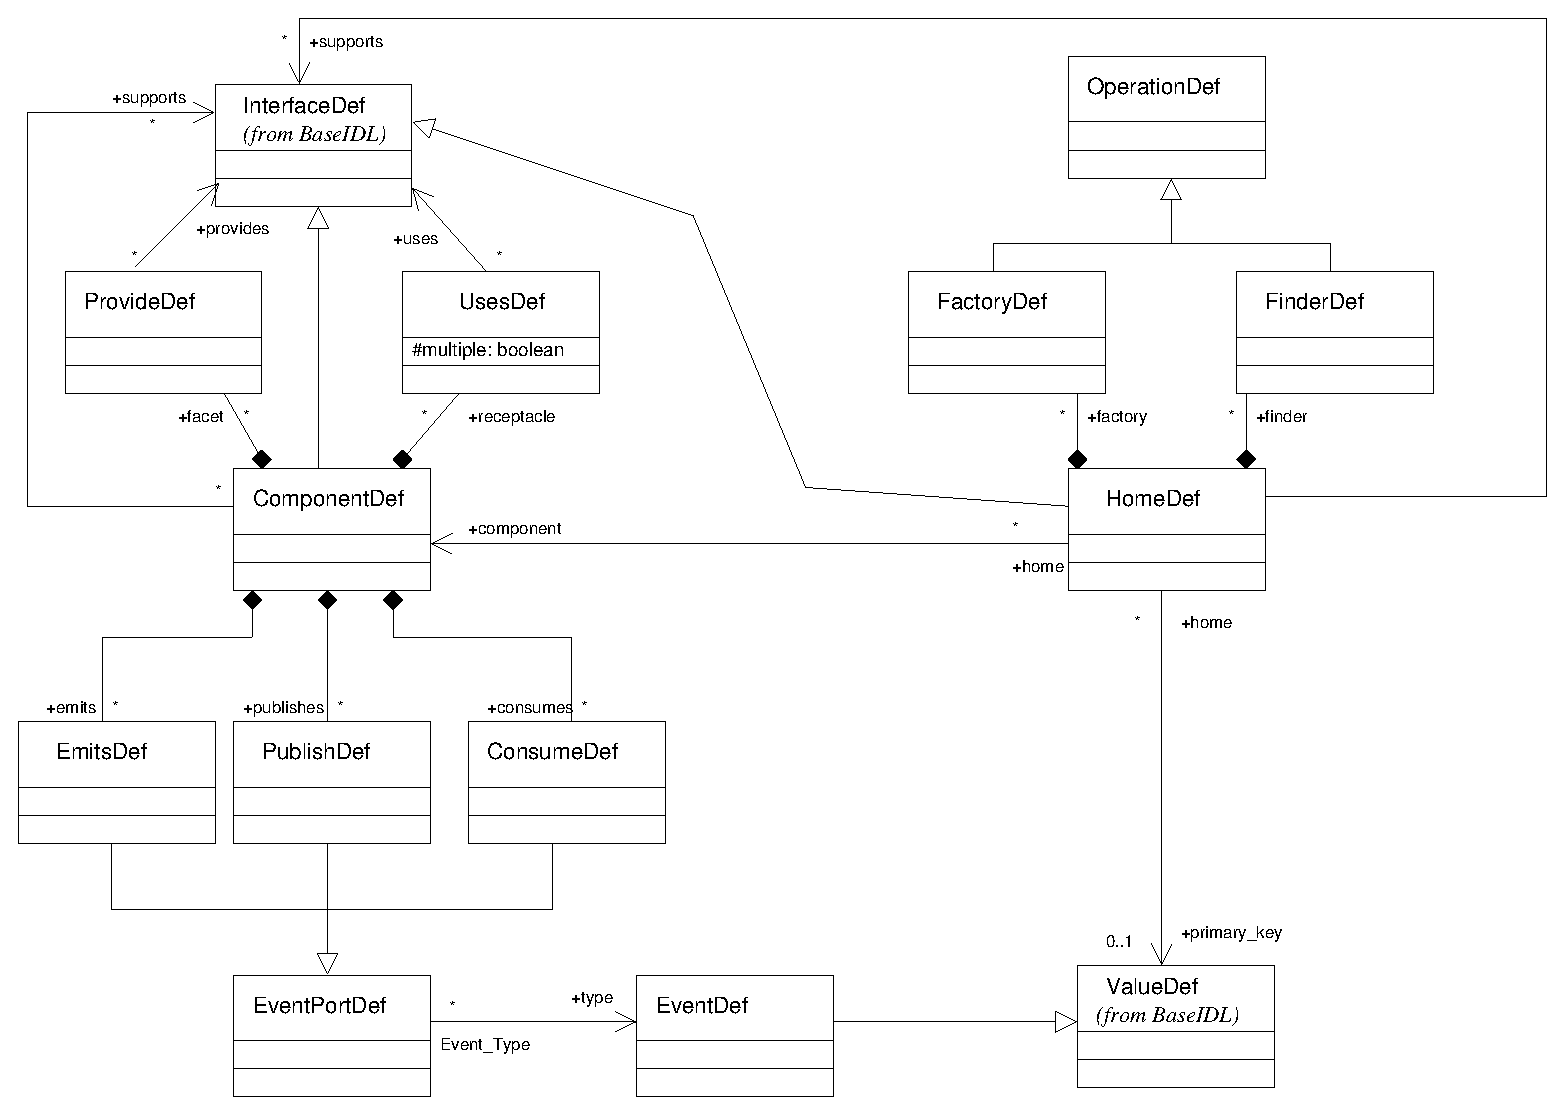
\includegraphics[width=\textwidth]{figures/fig-ccm-model.eps}
    \caption{Corba Component Model (fragment)}
    \label{fig-ccm-model}
\end{figure}

\paragraph{Le mod\`ele abstrait de composants}

Ce mod\`ele est pour l'essentiel la d\'efinition du langage \textsf{IDL3}, un
sur-ensemble du langage de description d'interface de \textsf{CORBA} qui ajoute
un certain nombre de mots cl\'es  permettant de d\'efinir la
structure logique des composant. Un composant est ainsi d\'efini
comme un ensemble d'interfaces fournies et requises, et
d'\'ev\'enements consomm\'es et produits, plus \'eventuellement
des attributs repr\'esentant les
propri\'et\'es configurables du composant. 

\`A chaque composant est
associ\'e une \emph{fabrique} de composants ou \emph{home} qui
est une interface d\'ecrivant les modalit\'es de cr\'eation et,
pour le cas des composants de type entit\'es, de recherche
d'instances de composants.
 Ces d\'eclarations sont projet\'ees en \textsf{IDL2} sous la forme 
d'interfaces \textsf{CORBA} pour pouvoir \^etre accessibles au
travers de l'\textsf{ORB}.
La figure \ref{fig-ccm-model} est un diagramme \textsf{UML}
repr\'esentant les \'el\'ements principaux du \textsf{CCM}.

 \paragraph{Le mod\`ele de programmation}

Il comprend la d\'efinition du langage \textsf{CIDL} ---~\emph{Component Implementation
Definition Language}~---, permettant de d\'efinir
l'implantation d'un composant, et de la plate-forme d'ex\'ecution des
composants (les \emph{containers}). Quatre types de composants sont
d\'efinis : 
\begin{itemize}
\item les composants \textbf{service} ne maintiennent aucun \'etat entre 
  deux appels de m\'ethodes et ne poss\`edent pas d'identit\'e
  propre. Ils sont l'\'equivalent des \emph{EJB Session} sans \'etat ;
\item les composants  \textbf{session} maintiennent un \'etat pour la
  dur\'ee d'une \emph{conversation} avec un client, c'est \`a dire une
  succession d'invocations de m\'ethodes. Lorsque la session est
  termin\'ee --- le plus souvent sur d\'ecision du client, le composant
  perd son identit\'e. Ils sont l'\'equivalent des \emph{EJB Session} avec
  \'etat ;
\item les composants \textbf{processus} persistent entre deux
  invocations mais n'ont pas d'identit\'e. Ils n'ont pas
  r\'eellement d'\'equivalent sur \textsf{J2EE} ;
\item les composants \textbf{entit\'e}, enfin, qui ont un \'etat
  persistant et qui de plus poss\`edent une identit\'e propre au travers
  d'une cl\'e primaire. 
\end{itemize}

\`A chaque type de composant est associ\'e un type de \emph{container} qui 
se charge de la gestion des aspects non fonctionnels ---~persistance,
contexte transactionnel, s\'ecurit\'e, cycle de
vie~--- du composant et du routage des invocations effectu\'ees par les
clients. Les interfaces entre composants et containers sont g\'en\'er\'ees
automatiquement lors de la phase de compilation de la description \textsf{CIDL}. 
Un composant peut \^etre r\'ealis\'e par plusieurs objets au sens
\textsf{CORBA}, les \emph{ex\'ecuteurs}, qui chacun aura la charge d'une partie des
interfaces du composant, \`a charge pour le conteneur d'orchestrer la
cr\'eation des diff\'erentes instances d'objet et leur assemblage.

\paragraph{Le mod\`ele de d\'eploiement}

Le d\'eploiement d'un ou plusieurs composants est d\'ecrit par un
fichier \textsf{XML} qui d\'efinit la mani\`ere d'utiliser un composant 
ou un ensemble de composants en terme d'architecture logicielle et 
de contraintes syst\`emes. Ce \emph{descripteur} est  associ\'e au code du composant  dans un
fichier de d\'eploiement ---~une archive \texttt{.jar}, par exemple~--- qui 
est alors utilisable pour le d\'eveloppement d'une application
compl\`ete. 
Le logiciel de
d\'eploiement utilise ces informations pour dialoguer avec des
serveurs d'assemblage et d'installation afin de mettre en \oe uvre
les composants.

\paragraph{Critiques}

Le \textsf{CCM} reprend dans son mod\`ele abstrait les concepts
principaux des \textsf{ADL} : composants \`a  multiples interfaces,
connecteurs, fabriques de composants. Comme pour les autres
plateformes, le conteneur est l'\'el\'ement cl\'e qui isole le
composant des d\'etails des services techniques. Cette plateforme est
\`a notre avis la plus proche d'une architecture \`a base de
composants et nous nous en sommes d'ailleurs fortement inspir\'es
pour d\'efinir notre mod\`ele de composant (voir chapitre
\ref{chap-fidl}). La r\'ealisation concr\`ete de logiciels bas\'es
sur le \textsf{CCM} reste encore une t\^ache ardue, probablement par
le fait du manque d'outils permettant de s'abstraire des contingences
de l'\textsf{ORB}.

\subsection{Containers de composants}

Les  principaux intergiciels orient\'es composants que nous avons
d\'ecrits succintement ci-dessus sont des plateformes compl\`etes,
complexes et globalement difficiles \`a ma\^{\i}triser de par l'ampleur
des domaines qu'elles essayent de recouvrir. La principale
difficult\'e que l'on rencontre dans la mise en \oe uvre concr\`ete
de ces plateformes est la
quasi-impossibilit\'e dans laquelle se trouvent le concepteur et le
d\'eveloppeur de  s'abstraire des contraintes techniques induites par
les supports d'ex\'ecution et les outils. 

Dans le cas de \textsf{CORBA/CCM},
le d\'eveloppeur se trouve confront\'e \`a un mod\`ele
satisfaisant, suffisamment riche et conceptuellement clair, mais dont
les b\'en\'efices en termes de conception se trouvent quasiment
an\'eantis par la difficult\'e de mise en \oe uvre technique,
quelles que soient les plateformes --- j'ai eu l'occasion
d'exp\'erimenter les plateformes \textsf{OpenCCM} et \textsf{Mico/CCM}. Dans le cas de
\textsf{J2EE}, le probl\`eme de la complexit\'e technique reste entier encore
qu'un peu all\'eg\'e par rapport \`a CORBA, mais par contre le
mod\`ele de composants n'est pas satisfaisant et trop pauvre pour
supporter r\'eellement une conception orient\'ee composants. Enfin,
\`a l'exception de \textsf{.Net}, aucune de ces plateformes ne
supporte la notion pourtant essentielle de \emph{composite}.

R\'ecemment sont apparus un certain nombre de \emph{frameworks} 
dont l'objectif, plus ou moins inspir\'e par les travaux sur
l'\emph{Ing\'enierie Dirig\'ee par les Mod\`eles} ---
\emph{Model Driven Engineering} --- et les \textsf{ADL}, est de permettre
d'une part de construire r\'eellement l'application comme un
assemblage potentiellement hi\'erarchique de composants aux
d\'ependances explicites, d'autre part de ne faire payer aux
d\'eveloppeurs que ce qu'ils utilisent effectivement de
l'infrastructure technique. 

\subsubsection{Spring, Kilim \& PicoContainer}

Ces trois \emph{conteneurs de composants}, r\'ealis\'es initialement en
\textsf{Java} mais depuis partiellement port\'es sur \textsf{.Net}, partagent une m\^eme approche du probl\`eme qui peut
se r\'esumer par la mise en \oe uvre de la notion du \emph{design
  pattern} \og \emph{injection
  de d\'ependances}\fg , bien qu'ils soient tr\`es diff\'erents dans leurs
ambitions. La notion d'\emph{injection de d\'ependances} est un
terme invent\'e par Martin Fowler pour d\'ecrire un patron
de conception orient\'e-objet dans lequel les d\'ependances des
objets entre eux sont remplac\'ees par des d\'ependances vers des
abstractions, c'est \`a dire en \textsf{Java} des interfaces.


 Le plus l\'eger des trois, \textsf{Picocontainer} se veut
un framework extr\^emement simple permettant de 
construire des applications con\c{c}ues comme des assemblages de
composants \`a partir d'objets standards en \textsf{Java}
(POJO). Il offre diff\'erentes implantations de conteneurs et une API
minimaliste permettant d'assembler dynamiquement des instances
d'objets, les \emph{composants}, par d\'ecouverte de leurs
d\'ependances et de leurs interfaces, d\'ecouverte rendue possible
par l'utilisation des capacit\'es r\'eflexives des langages
d'implantation.

\textsf{Kilim} est bas\'e sur le m\^eme principe mais ajoute la
possibilit\'e de d\'ecrire les assemblages et la configuration des
composants dans un descripteur externe qui sera charg\'e par le
moteur au lancement  de l'application.

\textsf{Spring} enfin, est le plus complet  de ces frameworks et se
veut une infrastructure transversale destin\'ee \`a faciliter le
d\'eveloppement d'applications \textsf{J2EE} en implantant un mod\`ele de
composants. Comme pour les pr\'ec\'edents projets
cit\'es, Spring utilise l'\emph{injection de d\'ependances} pour
r\'ealiser au moment de son d\'eploiement des assemblages de
composants, composant \'etant ici comme pr\'ec\'edemment synonyme
d'objet.

\subsubsection{Fractal}
\label{sec:fractal}
Fractal est un mod\`ele de composant d\'ecoupl\'e de toute
implantation concr\`ete et qui pr\'esente un certain nombre de
caract\'eristiques originales. Le mod\`ele de base d\'etaill\'e
dans \cite{fractal-spec} se pr\'esente comme un ensemble
d'interfaces  d\'efinissant les exigences 
que doit remplir toute impl\'ementation du mod\`ele. Un composant
est ici compos\'e d'un \emph{contr\^oleur} ou  \emph{membrane} et de
sous-composants, \'eventuellement \emph{partag\'es} entre diff\'erents
composites. Les composants interagissent au moyen d'\emph{interfaces}
qui peuvent \^etre \emph{externes} ou \emph{internes} --- accessibles
uniquement aux composants encapsul\'es. Des interfaces de contr\^ole
g\'en\'eriques sont d\'efinies permettant d'offrir des
m\'ecanismes d'introspection, de liaison dynamique et de gestion du
cycle de vie.

Les caract\'eristiques les plus originales du mod\`ele sont : 
\begin{itemize}
  \item la s\'eparation d'un composant entre son corps et sa
    \emph{membrane} qui permet
    de d\'efinir de v\'eritables comportements pour l'interface d'un
    composant ou d'une architecture de composants, sans pr\'ejuger de
    son implantation. On peut ainsi d\'efinir des \emph{membranes}
    g\'erant la s\'ecurit\'e, des membranes filtrant ou retraitant
    les messages, des membranes poss\'edant tel ou tel
    service ;
  \item la prise en compte explicite des \emph{composites} comme des
    composants \`a part enti\`ere. Un composant peut
    \'eventuellement offrir des interfaces d'administration sur sa
    structure, ou la laisser totalement opaque ;
  \item le \emph{partage} des composants entre diff\'erents assemblages.
\end{itemize}

Ce mod\`ele poss\`ede une implantation de r\'ef\'erence en
\textsf{Java} d\'enomm\'ee \textsf{Julia} et a servi aussi \`a la
r\'ealisation de composants permettant de construire une sorte d'\emph{OS
en kit}. Il est au centre de plusieurs travaux de recherche et
poss\`ede une communaut\'e de d\'eveloppement relativement
active au travers du consortium \textsf{ObjectWeb}.

Le mod\`ele \textsf{Fractal} est int\'eressant ne serait-ce que par sa
relative \'economie de moyens lorsqu'on le compare aux plateformes
classiques. \`A notre avis, seule toutefois la d\'efinition explicite
de composites est r\'eellement un atout : la notion de membrane,
intellectuellement s\'eduisante n'est qu'une reformulation des
connecteurs et n'est pas un concept primitif d'architecture car il est
toujours possible de la remplacer par des familles de composants
sp\'ecifiques. Le partage de composants, quant \`a lui, pose des
probl\`emes de formalisation des d\'ependances, de
contractualisation des interactions et d'encapsulation des assemblages.

\section{Langages de Description \& de Conception d'Architecture}
\label{sec:lang-de-descr}

La pr\'ec\'edente section \'etait d\'edi\'ee aux plateformes et
outils pour la manipulation concr\`ete de composants. Nous remontons
d'un cran dans l'abstraction en examinant quelques propositions
permettant de concevoir des architectures de composants. La
premi\`ere partie est consacr\'ee aux langages de conceptions
g\'en\'eralistes. Leur caract\'eristique commune est de couvrir un
spectre tr\`es large de situations et par cons\'equent d'avoir une
s\'emantique relativement faible pour la mod\'elisation du
comportement des composants. La deuxi\`eme partie s'int\'eresse plus
particuli\`erement aux \textsf{ADL} sp\'ecialement con\c{c}us pour
repr\'esenter des architectures et des composants.

\subsection{UML}
\label{sec:uml}
\textsf{UML} est aujourd'hui l'outil de base pour la conception et
l'analyse des applications, gr\^ace \`a la simplicit\'e de ses
concepts de base et \`a la profusion d'outils existants pour
manipuler des mod\`eles. Le point fort d'\textsf{UML}, sa versatilit\'e, est  aussi son point faible : l'actuelle norme 2.0 est encore
en phase d'adoption au sein du consortium \textsf{OMG} et
l'int\'egration de la multitude de diagrammes disponibles ainsi que
le flou entourant leur s\'emantique rendent l'implantation
d'un processus r\'eellement dirig\'e par les mod\`eles encore
tr\`es difficile.

La notion de \emph{composant} est pr\'esente dans les versions
pr\'ec\'edentes du langage uniquement comme repr\'esentation d'une
entit\'e concr\`ete du syst\`eme d\'eploy\'ee sur une
architecture physique. Cette notion a \'et\'e \'etendue \`a celle
d'unit\'e de composition architecturale avec l'introduction des
\emph{diagrammes de composants}. Ces diagrammes, dont nous donnons un exemple tir\'e de la
sp\'ecification\cite{uml20-comp} dans la figure
\ref{fig-uml20-comp-sample}, permettent d\'esormais de repr\'esenter
explicitement des architectures de composants.

\begin{figure}[htbp]
    \centering
    \includegraphics[width=.9\textwidth]{figures/fig-uml20-comp-sample.eps}
    \caption{Exemple de diagramme de composants UML 2.0}
    \label{fig-uml20-comp-sample}
\end{figure}

De plus, il est d\'esormais possible d'attacher aux ports des
composants des sp\'ecifications de \emph{protocole} sous la forme de
\emph{State Machines} ce qui permet d'utiliser \textsf{UML} comme un \textsf{ADL} \`a
part enti\`ere. 

Ces diagrammes ont le m\'erite d'\^etre simples dans leurs principes
et de ne pas surcharger le langage. Les composants peuvent \^etre
d\'etaill\'es au moyen de la syntaxe \textsf{UML} existante :
diagrammes de classes, diagrammes d'\'etats-transitions. La notion
de connexion reste toutefois confondue avec celle de d\'ependance et
seuls les ports de type synchrone sont pris en compte
explicitement. 

\subsubsection{EDOC}
\label{sec:edoc}
\textsf{EDOC} --- \emph{Enterprise Distribued Object Computing} ---
est  un profil UML, c'est \`a dire une
sp\'ecialisation du langage UML et de son m\'eta-mod\`ele pour
repr\'esenter des concepts sp\'ecifiques \`a un domaine
d'application, une technologie ou un processus. C'est une norme
adopt\'ee par l'\textsf{OMG} en 2001. \textsf{EDOC} est une
alternative int\'eressante car plus compl\`ete aux \emph{diagrammes
  de composants} pour la mod\'elisation d'architectures de
composants. 

Le c\oe ur de \textsf{EDOC} est constitu\'e de l'\emph{Architecture de Collaboration
de Composants}  qui d\'efinit les concepts
d'architecture, d'assemblage, de composants et d'interactions en
termes de mod\`eles \textsf{UML}. L'objectif affich\'e de ce mod\`ele est de
r\'epondre \`a diff\'erents probl\`emes : 
\begin{itemize}
  \item la composition r\'ecursive de composants pour mod\`eliser des
    syst\`emes \`a diff\'erents niveoux d'abstractions ;
  \item  la
    \emph{tra\c{c}abilit\'e} de l'\'evolution des mod\`eles et des
    implantations, l'automatisation du processus du d\'eveloppement
    au travers d'une d\'emarche \textsf{MDA} ;
  \item  le couplage faible
    entre \'el\'ements d'un syst\`eme pour promouvoir la
    r\'eutilisation et l'\'evolution concurrente de diff\'erentes
    parties d'un syst\`eme ;
  \item  l'ind\'ependance envers les technologies ;
    \item et enfin l'\'emergence d'un march\'e des composants m\'etiers.
\end{itemize}
La figure \ref{fig-edoc-comp-sample} repr\'esente un
composite dans la notation \textsf{EDOC} ou \emph{processus
communautaire}  mod\'elisant un syst\`eme
d'achat-vente. Ce sch\'ema d\'etaille diff\'erents types de ports et
en particulier des \emph{multiports} ou protocoles.

\begin{figure}[htbp]
    \centering
    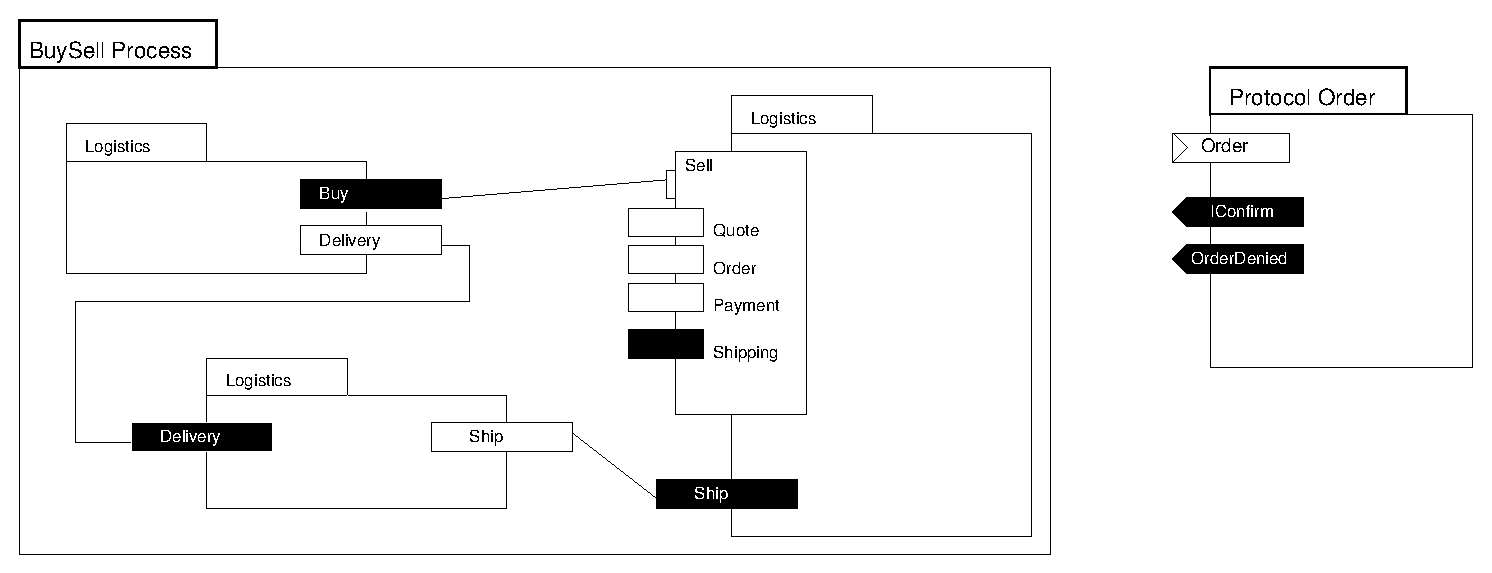
\includegraphics[width=.9\textwidth]{figures/fig-edoc-comp-sample.eps}
    \caption{Exemple de sch\'ema de composite EDOC}
    \label{fig-edoc-comp-sample}
\end{figure}

Les ports d'un composant sont :
\begin{itemize}
  \item soit des \'emetteurs ou r\'ecepteurs d'\'ev\'enements
  atomiques ;
\item soit des ports d\'efinissant un \emph{protocole d'interaction}
  dont le composant est l'initiateur ou le r\'epondeur,
  d\'ecrit au moyen d'un diagramme d'activit\'e ---une
  \emph{chor\'egraphie} dans la terminologie officielle --- et
  subdivis\'es eux-m\^emes en ports de granularit\'e plus fine. 
\end{itemize}
Si le mod\`ele de communication est au niveau le plus fin un
mod\`ele \emph{asynchrone} bas\'e sur des flots d'\'ev\'enements,
les protocoles permettent d'imbriquer des  s\'equences
d'\'ev\'enements et de protocoles pour constituer une
\emph{transaction} plus globale. Une \emph{op\'eration} au sens UML
du terme est vue comme un ensemble de flots li\'es par une
s\'emantique d'appel-retour.

Ce mod\`ele de base est \'etendu en un \emph{mod\`ele de processus
  m\'etiers} --- \emph{business process model} --- qui permet
de d\'efinir des 
processus concurrents communiquant par flots de donn\'ees en tant que composants.

Comme \`a l'accoutum\'ee, le document de normalisation est  tr\'es
pr\'ecis et d\'etaill\'e,  d\'ecrivant chacun des \'el\'ements
du profil, la notation associ\'ee, les contraintes stucturelles et la
s\'emantique de chacune des constructions. Cette proposition nous a
paru tr\`es int\'eressante, ne serait-ce que par ses objectifs qui
recouvrent une partie de nos pr\'eoccupations. Il
manque toutefois une formalisation explicite et compacte de la
s\'emantique des syst\`emes et architectures consid\'er\'es.

\subsubsection{AADL}

Le \emph{langage de conception et d'analyse d'architecture}\cite{aadl-overview} ---
\emph{Architecture Analysis \& Design Language} en anglais --- est une
proposition de standardisation de l'ing\'enierie dirig\'ee par les
mod\`eles et l'architecture pour les syst\`emes embarqu\'es
critiques d\'evelopp\'ee par la \emph{Society for  Automotive
  Engineers}. Cette proposition s'appuie sur les travaux de
normalisation de l'OMG dans le cadre de \textsf{UML 2.0} et les
travaux ant\'erieurs sur des outils de m\'eta-mod\'elisation tels
que \textsf{MetaH}.

\textsf{AADL} se pr\'esente essentiellement comme un socle commun de
concepts sur lequel pourront s'appuyer des outils de d\'eveloppement
et d'\'echange de mod\`eles, cibl\'e en direction de la
mod\'elisation de syst\`emes embarqu\'es. Il prend en compte 
la mod\`elisation des plateformes d'ex\'ecution au travers de
diff\'erents composants d'abstraction --- processeur, bus,
p\'eriph\'erique, m\'emoire ; et de composants logiciels parmi
lesquels on distingue des composants actifs --- \emph{threads}  et
processus --- et des composants passifs --- paquetages et donn\'ees.
\`A chaque composant peuvent \^etre attach\'ees des
\emph{propri\'et\'es} pr\'ed\'efinies ou sp\'ecifiques, et des
contraintes sur ces propri\'et\'es qui permettent de mod\'eliser et
v\'erifier des exigences \emph{temps-r\'eels}.

Les composants interagissent au travers de ports qui classiquement
isolent un composant des autres \'el\'ements du syst\`eme, ports
qui supportent trois modes de communication : le flot de donn\'ees
typ\'e avec une s\'emantique d'interruption --- au sens
d'interruption dans les syst\`emes d'exploitation --- ou de files, l'appel
de proc\'edure et le partage de variables.

Des outils existent, en particulier pour la plateforme
\textsf{Eclipse}, mais pour l'instant ils se limitent \`a
permettre la manipulation de mod\`eles au travers de diverses
interfaces  et des
v\'erifications de consistance interne des mod\`eles. \textsf{AADL} est
essentiellement une norme d'\'echange de mod\`eles, dont les forces
affich\'ees, la capacit\'e \`a int\'egrer des contraintes sp\'ecifiques aux
domaines et les points d'extension, nous paraissent \^etre
plut\^ot des inconv\'enients. Ce langage est en quelque sorte le
pendant pour le temps-r\'eel de \textsf{EDOC}. 

\subsection{ADL}

\cite{survey-long} propose une taxonomie des
principaux \textsf{ADL} selon plusieurs axes. Cette \'etude assez
large identifie les concepts du domaine et la mani\`ere dont chaque
langage les d\'efinit et 
permet de les manipuler. Nous avons choisi de nous int\'eresser dans les paragraphes qui suivent
\`a deux \textsf{ADL} non pr\'esent\'es dans cette \'etude et qui nous ont parus
pr\'esenter des caract\'eristiques proches de nos pr\'eoccupations
: \textsf{SOFA} et \textsf{ArchJava}. Toutefois, nous introduisons la
discussion avec une analyse de deux \textsf{ADL} \og classiques\fg
\textsf{Wright} et \textsf{Rapide}, parmi les premiers
\textsf{ADL} \`a supporter une s\'emantique formelle. 

\subsubsection{Wright \& Rapide}
\label{sec:wright}

\textsf{Wright}\cite{archcon} est \`a l'origine avec
\textsf{UniCon}\cite{shaw-abstract-archi}  de l'introduction de
\emph{connecteurs} formellement sp\'ecifi\'es entre composants,
c'est \`a dire de la d\'efinition de protocoles de communication
entre composants d'un syst\`eme. Les composants et connecteurs sont
sp\'ecifi\'es par des expressions \textsf{CSP}\cite{hoare-csp} avec la
s\'emantique en termes de traces et de refus de ce langage. Un
connecteur est vu comme l'ex\'ecution en parall\`ele de plusieurs
processus d\'ecrivant les \emph{r\^oles} dans lesquelles le
connecteur peut-\^etre utilis\'e et un processus \emph{colle}
d\'ecrivant les interactions entre r\^oles. Un composant est
d\'efini aussi par des expressions \textsf{CSP} d\'ecrivant ses diff\'erents
\emph{ports} et son comportement. 

La compatibilit\'e
entre r\^oles --- d'un connecteur --- et port --- d'un composant ---
et donc la correction d'une architecture donn\'ee, est assur\'ee par
la v\'erification d'une relation de \emph{raffinement} \'etendue
entre processus. Plus pr\'ecis\`ement, un port est compatible avec
un r\^ole si l'intersection des traces du port et des traces
d\'eterministes du r\^ole est un raffinement de l'ensemble de traces
du r\^ole. Une propri\'et\'e importante que l'on peut v\'erifier
est l'absence d'interblocage dans une configuration architecturale
donn\'ee. 

La motivation principale de \textsf{Wright} pour la
mod\'elisation explicite des connecteurs est d'exprimer
un nombre vari\'e de politique de communication. Elle
permet d'appliquer le formalisme sur une plus large gamme de syst\`emes en
d\'ecouplant la description des interactions de la description des
fonctionnalit\'es des composants. Les premi\`eres sont  
consid\'er\'ees g\'en\'eralement comme peu variables pour une
famille de syst\`emes donn\'ee  tandis que les seconds sont \emph{a
contrario} tr\'es variables. On notera, et c'est un point
aussi soulign\'e par les auteurs que l'on peut parvenir au m\^eme
r\'esultat en utilisant uniquement des composants et une seule
modalit\'e de communication.

Rapide \cite{rapide} est un syst\`eme complet de sp\'ecification et
de d\'eveloppement de syst\`emes distribu\'es orient\'es objets
guid\'e par l'architecture. Les composants sont des objets
concurrents, hi\'erarchiques, typ\'es par interfaces et implant\'es
par des modules. Ils communiquent par des connexions explicites en
\'emettant des \emph{actions} et invoquant des
\emph{fonctions}. L'ensemble des \'ev\'enements d'un syst\`eme
forme un ordre partiel d'\'ev\'enements qui constitue la base de la
s\'emantique d'ex\'ecution. 

Les  \emph{interfaces}  d\'efinissent des signatures d'actions et de
fonctions requises et fournies et \'eventuellement un \emph{contrat}
sous la forme de contraintes comportementales, sur le contenu des
messages \'echang\'es au travers de l'interface, et sur la
causalit\'e entre \'ev\'enements re\c{c}us et \'emis par
l'interface. Une \emph{architecture} d\'efinit l'implantation
d'une interface en termes d'interfaces imbriqu\'ees et de leurs connexions. Les \emph{connexions}
d\'efinissent des relations de causalit\'e entre ordre partiels
d'\'ev\'enements soit entre \'ev\'enements externes, soit entre
\'ev\'enements externes et internes. La notion de service permet de
regrouper un ensemble d'\'ev\'enements dans un type et de connecter directement
des services compl\'ementaires. Enfin, la notion de \emph{mapping}
permet de d\'efinir des transformations d'un ensemble
d'\'ev\'enements dans un autre, offrant ainsi la possibilit\'e de
d\'ecrire des relations entre diff\'erents niveaux d'abstractions.
Les propri\'et\'es que l'on peut v\'erifier sont nombreuses : la conformit\'e d'une architecture par rapport \`a son
interface, d'une implantation par rapport \`a son architecture, des
propri\'et\'es sur les s\'equences d'\'ev\'enements, ...

\subsubsection{ArchJava}

ArchJava\cite{aldrich-archjava,aldrich-archjava-reasoning} est une
extension au langage \textsf{Java} similaire \`a un ADL permettant d'int\'egrer des
contraintes architecturales dans du code source. Les extensions au
langage permettent de v\'erifier des propri\'et\'es
d'\emph{int\'egrit\'e des communications} : les objets communiquent entre
eux uniquement par les ports sp\'ecifi\'es. Ces propri\'et\'es
sont v\'erifi\'ees \`a la compilation par une extension du
syst\`eme de type de Java int\'egrant les notions de ports, de
composants et de composites. On v\'erifie ainsi que des composants ne
peuvent communiquer qu'avec des membres d'un m\^eme composite, des
sous-composants ou le composant englobant. 

Un \emph{composant} est une instance d'une classe \texttt{component}
contenant des d\'efinitions de \emph{ports}. Un port est un ensemble
de m\'ethodes qui peuvent \^etre \emph{fournies}, \emph{requises} ou
\emph{diffus\'ees} (\emph{broadcast}). Les m\'ethodes fournies doivent
\^etre implant\'ees par le composant, les m\'ethodes requises
\'etant fournies par l'autre extremit\'e de la connexion. 

Un port peut \^etre d\'efini au moyen d'un type \emph{interface de
  port} contenant uniquement des signatures de m\'ethodes
  fournies, offrant ainsi la possibilit\'e de d\'efinir
  dynamiquement le composant implantant r\'eellement le port. 

Un \emph{composite} est un composant contenant d'autres composants et qui
d\'ecrit des connexions ou des sch\'emas de connexion autoris\'es
entre ses sous-composants, et \'eventuellement avec ses propres
ports. Un composite dispose de la capacit\'e d'invoquer directement
les m\'ethodes de ses sous-composants, l'inverse n'\'etant pas vrai.

Dans  \cite{aldrich-archjava-reasoning}, un mod\`ele formel du
langage ArchJava est d\'efini essentiellement au travers d'un syst\`eme de types
et d'une s\'emantique op\'erationnelle. Ce mod\`ele est
bas\'e sur FeatherweightJava \cite{featherweightjava}, une
formalisation du langage \textsf{Java} usuel. On
v\'erifie \`a l'aide de ce mod\`ele que l'int\'egrit\'e des communications est bien maintenue
par le typage et certaines instructions \`a l'ex\'ecution
(v\'erification du transtypage) :
\begin{itemize}
  \item un composant $C$ ne peut appeler directement des m\'ethodes
    d'un composant $C'$ que si $C=C'$ ou si $C'$ est un sous-composant
    de $C$ ;
  \item dans tous les autres cas, la communication entre composants se
    fait au travers de leurs ports.
\end{itemize}

Le principal int\'er\^et du mod\`ele \textsf{ArchJava} est sa
proximit\'e avec le langage \textsf{Java} ce qui permet d'int\'egrer
facilement des concepts architecturaux dans les d\'eveloppements, la
correction \'etant assur\'ee par le syst\`eme de types. C'est aussi
son principal inconv\'enient qui rend ce mod\`ele trop li\'e \`a
une impl\'ementation pr\'ecise --- en l'occurence un langage et une
plateforme d'ex\'ecution --- et surtout qui induit un glissement des
probl\'ematiques architecturales de la conception vers la
r\'ealisation ce qui n'est pas l'objectif souhait\'e. De plus, les
concepts de composants se t\'elescopent avec les concepts objets
usuels du langage ce qui peut rendre l'utilisation de ce syst\`eme
\`a grande \'echelle tr\`es d\'elicate. 

\subsubsection{SOFA}

Le mod\`ele \emph{SOFA} --- pour \emph{Software Appliances} --- est
d\'etaill\'e pour l'essentiel dans \cite{plasil-sofa} et fait
partie d'un projet plus large d'une plateforme de conception de
composants, par ailleurs int\'egr\'e dans le consortium
\emph{Objectweb}.  L'objectif du mod\`ele, qui emprunte la majeure
partie de ses concepts aux \textsf{ADL}, est de permettre la \emph{validation statique}
de syst\`emes de composants hi\'erarchiques, la validit\'e du raffinement
d'architecture dans l'\'etape de conception, et la v\'erification
dynamique au travers de l'embarquement d'assertions d\'eriv\'ees du
langage de sp\'ecification \`a l'ex\'ecution.

Le concept de base de \textsf{SOFA} est la notion de \emph{protocole} d\'efinissant un
langage sur un
alphabet compos\'e de messages de type requ\^ete-r\'eponse. Ce
langage est rationnel ou approch\'e par un rationnel. Un
protocole peut \^etre attach\'e \`a une \emph{connexion}, c'est
\`a dire un lien bidirectionnel entre deux entit\'es. Ou il
peut \^etre attach\'e  \`a un
\emph{agent}, c'est \`a dire une entit\'e utilisant une ou plusieurs
connexions pour communiquer avec son environnemnt. L'alphabet d'un
protocole est partitionn\'e entre un ensemble de messages
fournis  et un ensemble de messages requis.

Un \emph{cadre}  d\'efinit un ensemble
d'interfaces fournies et requises, une interface \'etant une
collection de m\'ethodes, et un protocole sur les alphabets induits
par ces interfaces. Une \emph{architecture} est la r\'ealisation d'un
cadre par un ensemble d'autres cadres et la d\'efinition de
connexions entre ceux-ci, autrement dit une structure sens\'ee
implanter le cadre. Ces deux \'el\'ements peuvent se combiner de
mani\`ere hi\'erarchique jusqu'\`a atteindre les composants
primitifs par d\'efinition indivisible.

La principale propri\'et\'e que l'on peut d\'efinir et v\'erifier
sur les diff\'erentes entit\'es composant un syst\`eme est la
notion de \emph{substituabilit\'e de protocole} qui permet de
s'assurer de la compatibilit\'e d'une architecture avec une frame et
des deux parties prenantes dans une connexion.  Cette propri\'et\'e
s'\'enonce informellent comme $A$ est substituable \`a $B$ si :
\begin{enumerate}
  \item  $A$ fournit au moins tous les services fournis par $B$ :
  \item et $A$ ne requiert pas plus de son environnement que n'en aurait
  exig\'e $B$ \emph{dans les m\^emes conditions}.
\end{enumerate}

\section{Sp\'ecification formelles \& composants}

Cette derni\`ere section est consacr\'ee \`a des mod\`eles tr\`es
th\'eoriques prenant en compte des probl\'ematiques de composition et de
connexions de composants. 

\subsection{\pc et Alg\`ebres de processus}

Le \pc\cite{calcmp1,calcmp2} est une alg\`ebre de processus
destin\'ee \`a mod\'eliser et
\'etudier les propri\'et\'es des syst\`emes distribu\'es. Ce
formalisme se distingue de ses pr\'ecurseurs et de ses successeurs par une
remarquable \'economie de moyens syntaxiques et une expressivit\'e
non moins remarquable. 
L'\'el\'egance et l'expressivit\'e  du
langage proviennent de l'uniformit\'e de traitement offerte par la
notion de \emph{noms}, un terme tr\`es abstrait qui est \`a la fois une
variable, un identifiant de canal de communication et une donn\'ee
que l'on peut \'echanger. 

La notion d'\'equivalence comportementale est captur\'ee par le
concept de \emph{bisimulation}, relation fondamentale entre les termes
du \pc et que nous retrouverons dans
le chapitre \ref{chap-etatarttest} consacr\'e au test de composants. Le principal
inconv\'enient du \pc est aussi son principal avantage : sa
\emph{puissance}. Cette puissance  induit \emph{de facto}
l'ind\'ecidabilit\'e de la plupart des propri\'et\'es
int\'eressantes dans le cas de la version g\'en\'erale du langage
 et en particulier de
l'\'equivalence comportementale des termes, donc de la relation de
bisimulation. La sobri\'et\'e de la syntaxe et de la s\'emantique
rendent inutilisable le \pc autrement que comme objet de r\'eflexion
th\'eorique, et c'est pourquoi de nombreux travaux ont cherch\'e
\`a accro\^{\i}tre son \og \emph{utilisabilit\'e}\fg, par exemple au
travers de calculs polyadiques, de l'introduction de types primitifs
et d'un syst\`eme de types sur les termes.

\subsubsection{Piccola}
\textsf{Piccola} est un langage de composition d\'evelopp\'e par le
\emph{Software Composition Group} de
Berne\cite{piccola,formallangcomp,compsoftres}. Bien qu'il ne
s'agisse pas \`a proprement parler d'une plate-forme de composants,
cette approche nous semble int\'eressante car elle met l'accent sur la
notion de connecteurs, r\'eifi\'es sous la forme de scripts
\textsf{Piccola}. Ces scripts permettent \`a des composants \'ecrits
simplement en \textsf{Java} de s'\'echanger des donn\'ees structur\'ees
---~appel\'ees \emph{forms}~--- en s'abstrayant de l'architecture
mat\'erielle et logicielle de l'application. La s\'emantique du
langage est bas\'ee sur une version du \pc, le \pc asynchrone
polyadique dans lequel les op\'erations de communication peuvent
mettre en \oe uvre des n-uplets de noms et sont r\'ealis\'ees  de
mani\`ere asynchrone. Il ne semble pas
toutefois que ces d\'eveloppements s'int\'eressent \`a la v\'erification et \`a la validation de
programmes autrement qu'au moyen d'un syst\`eme de types\cite{regtypes}. 

\subsubsection{Darwin}

\textsf{Darwin}\cite{darwin} est  un \textsf{ADL} qui
permet de d\'efinir des architectures de composants inter-connect\'es
et hi\'erarchiquement structur\'es, et dans lequel la s\'emantique
des op\'erations de connexion est d\'efinie au moyen de termes du
\pc polyadique synchrone. L'id\'ee centrale consiste \`a attacher
\`a chaque port de service fourni et requis un terme du \pc et, \`a
partir d'une configuration donn\'ee, de v\'erifier par application
des r\`egles de r\'eduction du calcul que la configuration est
correcte, c'est \`a dire que chaque port requis se trouve connect\'e
au bon port fourni. Ce principe de base est \'etendu au probl\`eme
de la cr\'eation de nouvelles instances de composants, cr\'eation
qui est exprim\'ee aussi comme un terme du \pc et dont la
s\'emantique permet de v\'erifier \`a la
conception  et \`a l'ex\'ecution sa viabilit\'e en fonction d'un contexte. Notons que ce
langage ne s'int\'eresse pas au fonctionnement des
composants ni \`a la sp\'ecification de leurs services mais
uniquement \`a la validation d'une structure donn\'ee. 

\subsubsection{CORBA \& \pc}

Les travaux de \cite{refinepi,picorba} utilisent le
\pc pour sp\'ecifier le comportement d'interfaces CORBA et
\cite{canal-compat-arch} en d\'etaillent les aspects formels. Le
comportement d'interfaces --- roles --- et de composants d'un
syst\`eme est sp\'ecifi\'e sous la forme d'agents du \pc, et une
relation de \emph{compatibilit\'e} entre agents est propos\'ee
permettant de v\'erifier la conformit\'e de deux interfaces entre
elles dans l'optique par exemple d'adapter  le comportement de l'une
\`a l'autre et de pouvoir d\'eriver automatiquement des
\emph{adaptateurs} et connecteurs poss\'edant certaines
propri\'et\'es et compatibles avec une architecture donn\'ee.
Une \emph{relation de compatibilit\'e} permet de prouver que la composition de deux composants
au travers de leurs interfaces est correcte si les \emph{connexions}
entre interfaces sont compatibles, une propri\'et\'e importante que
nous \'etudierons dans le contexte qui est le notre au chapitre
\ref{cha:composition}. Enfin, une relation d'h\'eritage entre agents
et d'extension de comportement est d\'efinie qui pr\'eserve la
compatibilit\'e des interfaces. 

Dans \cite{bracciali-comp-adapt}, le probl\`eme de l'adaptation
automatique du comportement d'interfaces est \'etudi\'e dans le
cadre pr\'esent\'e ci-dessus. La technique utilis\'ee consiste \`a
construire incr\'ementalement un \emph{agent d'adaptation}, c'est \`a dire un terme du
\pc, \`a partir d'une application --- \emph{mapping} --- entre les
signatures et les contraintes de chacune des interfaces \`a adapter,
de sorte que le nouvel agent compos\'e avec les deux agents initiaux
produise un comportement correct.

Le choix du \pc est ici, comme pour les travaux
pr\'ec\'edemment cit\'es, guid\'e par la capacit\'e de cette
th\'eorie \`a mod\'eliser facilement la mobilit\'e et la dynamique
structurelle des syst\`emes. 
Il n'est bien s\^ur pas le seul formalisme de la famille des
alg\`ebres de processus \`a avoir \'et\'e utilis\'e pour
sp\'ecifier le comportement d'architectures logicielles : l'\textsf{ADL}
\emph{Wright}, par exemple, (voir  section \ref{sec:wright}) utilise
\textsf{CSP} comme outil de sp\'ecification de comportements et le
\emph{kell-calcul} est une variante complexe du calcul des ambients pour
d\'efinir une s\'emantique formelle \`a la plateforme \textsf{Fractal}.
 
\subsubsection{M-Calcul \& Kell-Calcul}

Le \textsf{M-calcul}\cite{M-calcul} est un \emph{calcul de processus} inspir\'e de
pr\'ed\'ecesseurs tels que le \emph{calcul des ambients}, le
\emph{join-calculus}, le \emph{blue calculus}, la \emph{Chemical
  Abstract Machine}. C'est \`a dire qu'il s'int\'eresse non
seulement aux processus, \`a leurs compositions au travers
d'op\'erateurs alg\'ebriques, mais aussi \`a la notion, centrale
pour les mod\`eles \`a composants, d'encapsulation et de
structure. La principale entit\'e de ce calcul est la \emph{cellule}
qui, par analogie avec la cellule biologique, est constitu\'ee d'une
\emph{membrane}  et d'un \emph{plasme}, chacun \'etant d\'ecrit
comme  un processus.

Le point qui distingue le \emph{M-calcul} de ses concurrents est la
mani\`ere dont ont lieu les communications entre cellules. Les
cellules sont organis\'ees de mani\`ere hi\'erarchique \`a partir
d'une racine, le syst\`eme. La membrane agit comme un contr\^oleur
et un filtre sur les messages qui entrent  et sortent du plasme, ce qui
autorise toutes sortes de mod\'elisations de syst\`emes distribu\'es
complexes : firewalls, syst\`emes d'authentification, syst\`emes
tol\'erants aux pannes, r\'esolution dynamique de noms, ... 

Le \emph{kell-calcul}\cite{kell-calculus} est un raffinement du M-calcul dans
lequel ont disparu les concepts distincts de membrane et de plasme au
profit d'une vision plus uniforme de processus imbriqu\'es \emph{\`a la}
calcul des ambients.  La communication est rendue plus abstraite et
plus g\'en\'erale par l'utilisation d'un m\'ecanisme de
filtrage de motifs param\'etrant le
langage, d'o\`u la qualification du kell-calcul comme une famille
de langages. Ce filtrage op\`ere sur la structure des messages
\'echang\'es entre les diff\'erentes cellules ou \emph{kells} 
et peut \^etre arbitrairement complexe. L'objectif de
ce projet est de fournir une s\'emantique formelle, compl\'et\'ee
de l'arsenal usuel : syst\`eme de types, relations d'\'equivalences,
r\'esultats de d\'ecidabilit\'e, pour la plate-forme de composants
\textsf{Fractal} (voir section \ref{sec:fractal}).

\subsection{Composants \& Coalg\`ebres}

Les approches pr\'esent\'ees ci-dessous s'inscrivent dans la
th\'eorie des co-alg\`ebres d\'efinie en termes cat\'egoriques et
dont une synth\`ese est donn\'ee  dans \cite{coalgebra-tutorial}. La
notion de co-alg\`ebre \emph{dualise} la notion d'alg\`ebre et
permet de d\'efinir un cadre pour la sp\'ecification abstraite de
syst\`emes dynamiques au comportement infini, la comparaison par bisimulation et la preuve
par co-induction.

\subsubsection{Abstract Behavior Types \& \textsc{Reo}}

Le mod\`ele de composants propos\'e dans \cite{ABT} est bas\'e sur
la notion de \emph{type abstrait de comportement} d\'efini comme une
relation entre des \emph{flots de donn\'ees temporis\'es}
d'entr\'ee et de sortie. Informellement, les composants
mod\'elis\'es sont suppos\'es \'echanger des messages avec
leur \emph{environnement} au travers d'interfaces soit en entr\'ee,
soit en sortie. Une interface est un flot
de donn\'ee temporis\'e, c'est \`a dire une paire de s\'equences
infinies d'\'el\'ements d'un ensemble quelconque et
de r\'eels strictement croissants. Les
\'ev\'enements sont suppos\'es ordonn\'es, atomiques et
poss\`edent une dur\'ee non nulle. 

Un composant est ainsi un ensemble de flots de donn\'ees temporis\'es,
\'etiquet\'es comme entr\'ee ou sortie, et la relation existant
entre ces flots. Ce mod\`ele permet de donner une s\'emantique au
langage de composition \textsc{Reo} introduit par ailleurs dans
\cite{constraint-automata}.  Ce langage d\'efinit un ensemble de connecteurs
et de composants primitifs composables pour produire des syst\`emes plus larges. 

Un connecteur en \textsc{Reo} est un ensemble de \emph{canaux}
organis\'es en graphe o\`u les n\oe uds sont des regroupements de
points d'attaches de canaux et les arcs  entre deux n\oe uds
contenant les points d'attache du canal. Un canal est un medium de
communication entre deux points d'attache. Cet ensemble minimal de
d\'efinitions est compl\'et\'e par une op\'eration de regroupement
de points d'attache, ou \emph{join}, r\'eunissant plusieurs points
d'attache dans un seul n\oe ud, et une s\'emantique de transmission
des messages dans les n\oe uds qui permet en particulier de
r\'epliquer les messages sur tous les canaux li\'es \`a un point
d'attache.

L'int\'er\^et principal de cette approche est l'accent mis sur la
topologie abstraite des connecteurs et des n\oe uds. Cette structure
et ses op\'erateurs permettent de
d\'efinir des propri\'et\'es de coordination et de communication de
composants de mani\`ere \emph{exog\`ene}. Les composants eux m\^emes
n'ont besoin d'aucune connaissance sur les autres acteurs de leur
environnement et sont compl\`etement encapsul\'es.

\cite{coind-calc-component} pr\'esente cette m\^eme approche en la
reliant aux notions de bisimulation et de co-induction. La d\'efinition d'une relation de bisimulation permet
d'obtenir un principe de preuve pour l'\'equivalence de connecteurs,
principe qui peut \^etre utilis\'e pour la v\'erification de
protocoles ou pour optimiser un syst\`eme fait de connecteurs plus
simples. La s\'emantique op\'erationnelle de \textsc{Reo} est d\'efinie par
des \emph{automates de contraintes}, introduits dans
\cite{constraint-automata}. Ces contraintes sont des  gardes permettant de d\'efinir la relation existant entre les
  donn\'ees sur les diff\'erents ports de l'automate et des
  propri\'et\'es du flot temporel ordonnancant les donn\'ees.

On retrouve dans \textsf{Reo}, formalis\'es pour le temps-r\'eel,
tous les concepts des architectures  de composants : connecteurs,
interfaces et points  d'attache, composition et encapsulation. 

\subsubsection{Composants g\'en\'eriques et monades}

Une autre approche plus abstraite bas\'ee sur la th\'eorie des
co-alg\`ebres est pr\'esent\'ee dans
\cite{coalg-comp-proc,gen-comp,coalg-calc-comp}. Un composant est d\'efini par ses
entr\'ees, ses sorties et une certaine structure de
\emph{coalg\`ebre} d\'efinissant le comportement du composant par
les relations entre ses entr\'ees et ses sorties. Cette structure est param\'etrique au
sens o\`u pour un m\^eme composant on peut d\'ecrire diff\'erentes \emph{formes} du
syst\`eme de transition d\'ecrivant le comportement du composant,  au moyen de constructions
classiques dans la th\'eorie des cat\'egories\cite{maclane-categories}.

On peut d\'efinir de mani\`ere abstraite
une op\'eration d'encapsulation, transformant les ensembles
d'entr\'ees-sorties et diff\'erentes op\'erations de composition :
s\'equentielle, alternative  --- \emph{ie.} non-d\'eterminisme induit par
l'environnement ---  parall\`ele, synchronis\'ee. On notera que les
propri\'et\'es de ces op\'erations sont d\'ependantes des
caract\'eristiques de la structure param\'etrant le
comportement des composants observ\'es. Dans \cite{meng-coalg-uml},
cette approche est utilis\'ee pour formaliser la s\'emantique de
certains diagrammes \textsf{UML}, diagrammes de classe, cas d'utilisation et
diagrammes d'\'etats, et d\'ecrire des propri\'et\'es de
raffinement.

Pour int\'eressante qu'elle soit sur le plan th\'eorique, cette
approche est tr\`es \'eloign\'ee des probl\`emes pos\'es par le
d\'eveloppement d'architectures de composants, le terme m\^eme de
composant n'\'etant pas clairement rattach\'e \`a un concept
op\'erationnel. 

\section{Conclusion}

La r\'ealisation d'un mod\`ele d'architecture ex\'ecutable
susceptible d'\^etre utilis\'e pour v\'erifier et valider des
applications n\'ecessite de prendre en compte quatre concepts
cl\'es :
\begin{enumerate}
  \item les \emph{composants} qui forment les briques de base d'un syst\`eme
  ;
\item les \emph{donn\'ees} qui sont  l'information \'echang\'ee et
  transform\'ee par les composants ;
\item les \emph{ports} qui permettent d'assembler des composants et
  de faire transiter de l'information ;
\item les \emph{composites} qui permettent de produire \`a partir d'un ensemble
  de composants connect\'es par leurs ports un nouveau composant
  lui-m\^eme de nouveau composable.
\end{enumerate}
Les \emph{connecteurs} ne sont pas un concept primitif de l'architecture car
ils peuvent \^etre mod\'elis\'es \`a volont\'e par des
composants. Dans l'optique d'une applicabilit\'e directe du
mod\`ele, il para\^{\i}t toutefois important de conserver la
s\'emantique des appels de proc\'edures --- appels/retours li\'es
--- qui est la plus commune dans les plateformes concr\`etes m\^eme
si de nombreux mod\`eles font le choix de se limiter au passage de
messages. Le mod\`ele de communication est \emph{in fine} peu
important puisqu'il est toujours possible de simuler des
communications synchrones avec des mod\`eles asynchrones et
vice-versa. Un mod\`ele asynchrone nous semble toutefois plus simple
\`a mettre en \oe uvre si l'on souhaite d\'efinir des politiques
d'ordonnancement et de distribution particuli\`ere des messages et
offre une s\'emantique  plus proche de la r\'ealit\'e des syst\`emes r\'epartis. 

La formalisation en termes de langages de traces ou d'automates est le
meilleur moyen d'exprimer le comportement des ports, composants et
composites, sous r\'eserve de disposer d'un mod\`ele de composition
ad\'equat garantissant le maintien de propri\'et\'es des
ports. Les ports doivent donc \^etre des interfaces contractuelles
avec une distinction nette entre les entr\'ees et les sorties, les
premi\`eres \'etant d\'ependantes du contexte et les secondes du
composant mod\'elis\'e, leur r\^ole dans le contrat ne saurait
\^etre identique. Le choix d'un mod\`ele \`a base d'automates
d'\'etats finis permet par ailleurs de r\'ealiser facilement une
version ex\'ecutable d'une sp\'ecification et de plus, comme nous le
verrons au chapitre suivant, permet de construire des suites de
tests bas\'ees sur les nombreux travaux du test de conformit\'e de
protocole. 

%%% Local Variables: 
%%% mode: latex
%%% TeX-master: "these"
%%% TeX-master: "these"
%%% TeX-master: "these"
%%% TeX-master: "these"
%%% TeX-master: "these"
%%% End: 
